%%%%%%%%%%%%%%%%%%%%%%%%%%%%%%%%%%%%%%%%%%%%%%%%%%%%%%%%%%%%%%%%%
%%% %
%%% % weiiszablon.tex
%%% % The Faculty of Electrical and Computer Engineering
%%% % Rzeszow University Of Technology diploma thesis Template
%%% % Szablon pracy dyplomowej Wydziału Elektrotechniki 
%%% % i Informatyki PRz
%%% % June, 2015
%%%%%%%%%%%%%%%%%%%%%%%%%%%%%%%%%%%%%%%%%%%%%%%%%%%%%%%%%%%%%%%%%

\documentclass[12pt,twoside]{article}

\usepackage{weiiszablon}
\usepackage{hyperref}

\author{Mateusz Fesz}

% np. EF-123456, EN-654321, ...
\studentID{EF-167788}

\title{Implementacja wielowarstowej sieci neuronowej oraz algorytmu wstecznej propagacji błędu z adaptacyjnym współczynnikiem uczenia. Badanie wpływu metaparametrów sieci na efektywność uczenia}
\titleEN{Temat pracy po angielsku}


%%% wybierz rodzaj pracy wpisując jeden z poniższych numerów: ...
% 1 = inżynierska	% BSc
% 2 = magisterska	% MSc
% 3 = doktorska		% PhD
%%% na miejsce zera w linijce poniżej
\newcommand{\rodzajPracyNo}{0}


%%% promotor
\supervisor{(tytuł naukowy przed) Imię i nazwisko opiekuna (tytuł po)}
%% przykład: dr hab. inż. Józef Nowak, prof. PRz

%%% promotor ze stopniami naukowymi po angielsku
\supervisorEN{(academic degree) Imię i nazwisko opiekuna}

\abstract{Treść streszczenia po polsku}
\abstractEN{Treść streszczenia po angielsku}

\begin{document}

% strona tytułowa
\maketitle

\blankpage

% spis treści
\tableofcontents

\clearpage
\blankpage

\section{Opis projektu}
\subsection{Cel projektu}
Celem projektu jest realizacja uniwersalnej sieci neuronowej wielowarstwowej oraz zbadanie wpływu metaparametrów sieci na przebieg i efektywność procesu uczenia.
Metaparametry poddane badaniom to:
\begin{itemize}
	\item S1 - liczba neuronów w pierwszej warstwie sieci
	\item S2 - liczba neuronów w drugiej warstwie sieci
	\item lr - współczynnik uczenia sieci
	\item er - współczynnik maksymalnego dopuszczalnego przyrostu błędu, oznaczany również jako MAX\_PERF\_INC
	\item lr\textsubscript{dec} - modyfikator współczynnika uczenia w przypadku przekroczeniu maksymalnego dopuszczalnego przyrostu błędu
	\item lr\textsubscript{inc} - modyfikator współczynnika uczenia w przypadku spadku błędu
\end{itemize}

\subsection{Opis i przygotowanie wykorzystanych danych}
W celu przeprowadzenia badań, wykorzystany został zbiór danych dostępny pod adresem: \url{https://archive.ics.uci.edu/ml/datasets/zoo}.
Składa się na niego 101 rekordów opisanych 18 parametrami. Opisują one następujące cechy zwierzęcia:
\begin{enumerate}
	\item animal name - wartość tekstowa, stanowiąca nazwę zwierzęcia. Nieuwzględniana w procesie uczenia
	\item hair - wartość logiczna, określająca występowanie owłosienia na ciele zwierzęcia
	\item feathers, wartość logiczna, stwierdzająca występowanie piór na ciele zwierzęcia
	\item eggs - wartość logiczna, niosąca informację o składaniu przez zwierzę jaj
	\item milk - wartość logiczna, określająca zdolność zwierzęcia do wytwarzania mleka
	\item airborne - wartość logiczna, stwierdzająca zdolność zwierzęcia do lotu
	\item aquatic - wartość logiczna, niosąca informację o zdolności zwierzęcia do funkcjonowania w środowisku wodnym
	\item predator - wartość logiczna, informująca czy zwierzę jest drapieżnikiem
	\item toothed - wartość logiczna, określająca występowanie uzębienia u zwierzęcia
	\item backbone - wartość logiczna, stwierdzająca występowanie kręgosłupa
	\item breathes - wartość logiczna, niosąca informację o sposobie oddychania zwierzęcia
	\item venomous - wartość logiczna, określająca czy zwierzę jest jadowite
	\item fins - wartość loiczna, stwierdzająca występowanie płetw
	\item legs - wartość liczbowa, informująca o liczbie nóg danego zwierzęcia
	\item tail - wartość logiczna, niosąca informację o występowaniu ogona
	\item domestic - wartość logiczna, określająca czy zwierzę jest uznawane za domowe
	\item catsize - wartość logiczna, o niesprecyzowanej informacji
	\item type - wartość liczbowa, określająca przynależność zwierzęcia do jednej z siedmiu klas
\end{enumerate}

W procesie uczenia należy dokonać dopasowania zwierzęcia do odpowiedniej klasy.
Jako parametry przyjmuje się kolumny 2-17.
Kolumna 18 zawiera oczekiwaną wartość klasyfikacji.
Kolumna pierwsza nie jest wykorzystywana w procesie uczenia, gdyż nie opisuje ona fizycznej cechy zwierzęcia, a jedynie jego nazwę.

Przed przystąpieniem do procesu uczenia, przeprowadzono normalizację danych wejściowych. Wymagała jej jedynie kolumna ,,legs'' przyjmująca wartości numeryczne z zakresu $[0;8]$.
Numer klasy stanowiący jedyną daną wyjściową został natomiast przekształcony do postaci siedmio-elementowego wektora, zawierającego wartość $1$ na pozycji odpowiadającej danej klasie oraz wartości $0$ na pozostałych pozycjach.
W ostatnim kroku, dokonano podziału danych na zbiór uczący oraz zbiór walidacyjny.
W tym celu przydzielono $25\%$ rekordów należących do danej klasy do zbioru walidacyjnego, zaś pozostałą część do zbioru uczącego.

\section{Zagadnienia teoretyczne związane z wykorzystaną siecią neuronową oraz algorytmem uczenia}
\subsection{Model neuronu}
Neuron jest podstawowym elementem sieci neuronowej.
Jego elementami są:
\begin{itemize}
	\item Zbiór wejść $x$ długości $L$
	\item Zbiór powiązanych z wejściami wag $w$ długości $L$
	\item Wartość przesunięcia $b$
	\item Blok sumujący
	\item Funkcja aktywacji $f$
	\item Wyjście $a$
\end{itemize}


\begin{figure}[ht]
	\centering
	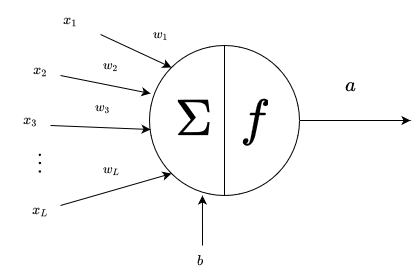
\includegraphics[width=12cm]{figures/models/neuronModel.png}
	\caption{Graficzny model neuronu}
	\label{Fig:neuron}
\end{figure}

Wartość sygnału wyściowego neuronu możemy określić wzorem:
\begin{equation}
	\label{eq:neuronOut}
	a = f\left(\sum\limits_{j=1}^{L}w_{j}x_{j} + b\right)
\end{equation}

W powyższym zapisie, $x_j$ oraz $w_j$ oznaczają odpowiednio kolejne wartości wejściowe i powiązane z nimi wagi (współczynniki wagowe).
Zapis ten możemy jednakże uprościć, zakładając że $x = \left[ x_1, x_2, ..., x_L\right]^T$ będzie wektorem kolumnowym wejść, $w = \left[ w_1, w_2, ..., w_L\right]$ - macierzą wierszową powiązanych z wejściami wag, natomiast wartości $a$ oraz $b$ - skalarami.
Wtedy równanie \ref{eq:neuronOut} przyjmie postać:
\begin{equation}
	\label{eq:neuronVec}
	a = f\left( w x + b \right)
\end{equation}

Ponadto istotnym w dalszych rozważaniach elementem modelu neuronu jest wyjście z bloku sumującego.
Oznaczając je jako $z$ otrzymamy:
\begin{equation}
	\label{eq:z}
	z = \sum\limits_{j=1}^{L}w_{j}x_{j} + b
\end{equation}

Obliczona w ten sposób wartość, stanowi argument funkcji aktywacji neuronu.
Funkcja ta przekształca wartość $z$ na inną wartość uzależnioną od jej charakterystyki.
Na potrzeby projektu, przyjęto że rolę tę będzie pełniła funkcja sigmoidalna (logsig).
Jej wartość możemy obliczyć zgodnie ze wzorem:
\begin{equation}
	\label{eq:sigmoid}
	f(z) =  \frac{1}{1 +\exp(-z)}
\end{equation}

W procesie uczenia istotna będzie także wartość pochodnej tej funkcji w danym punkcie.
W przypadku funkcji sigmoidalnej można ją sprowadzić do następującej postaci:
\begin{equation}
	\label{eq:sigmoidPrime}
	f'(z) = f(z) * 1-f(z)
\end{equation}
Co istotne, argumentami tej funkcji są stałe oraz wyliczona wcześniej pochodna w punkcie.
Właściwość ta może być użyta do zmniejszenia liczby wykonywanych przez algorytm operacji.


\subsection{Sieć neuronowa jednowarstwowa}
Siecią neuronową jednowarstwową nazywamy taką sieć, w której neurony nie są połączone ze sobą bezpośrednio, a jedynie otrzymują dane na wejściu i podają wynik na wyjście.

\begin{figure}[ht]
	\centering
	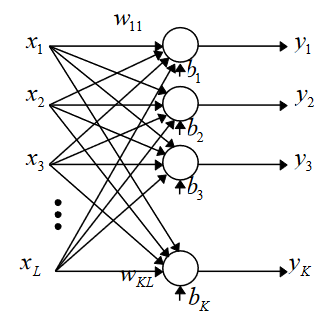
\includegraphics[width=12cm]{figures/models/singleLayerModel.png}
	\caption{Model prostej sieci jednowarstwowej - Placeholder}
	\label{Fig:singleNetwork}
\end{figure}

Wejściem każdego neuronu jest wektor sygnałów wejściowych $x$, zaś wyjściem sieci wektor $y = \left[ y_1, y_2, y_3, \cdots, y_L \right]^T$.
Ponadto możemy zdefiniować również wektor przesunięć $b = \left[ b_1, b_2, \cdots, b_K \right]$
Liczba wyjść z sieci jest tożsama z liczbą neuronów.

Wagi przyporządkowane wejściom można wyrazić w postaci macierzy o rozmiarach $K \times L$ gdzie $L$ oznacza liczbę wejść sieci, a $K$ liczbę neuronów.
$$\bm{w} = \left[
	\begin{array}{cccc}
		w_{11} & w_{12} & \cdots & w_{1L} \\
		w_{21} & w_{22} & \cdots & w_{2L} \\
		\vdots & \vdots &  & \vdots \\
		w_{K1} & w_{K2} & \cdots & w_{KL} \\
	\end{array}
	\right]$$

Przy założeniu że każdy neuron realizuje tą samą funkcję aktywacji, działanie sieci jednowartwowej wielowarstwowej możemy wyrazić w postaci macierzowej:
\begin{equation}
	\label{eq:singleLayerOut}
	y = f\left( wx + b \right)
\end{equation}
\subsection{Sieć neuronowa wielowarstwowa}
Siecią neuronową wielowarstwową, nazywamy taką sieć w której neurony ułożone są w dwóch lub więcej połączonych ze sobą warstwach.
Możemy zatem powiedzieć że jest to pewna liczba połączonych kaskadowo sieci jednowarstowych, a wyjście pojedynczej warstwy jest równocześnie wejściem warstwy następnej.
\begin{figure}[ht]
	\centering
	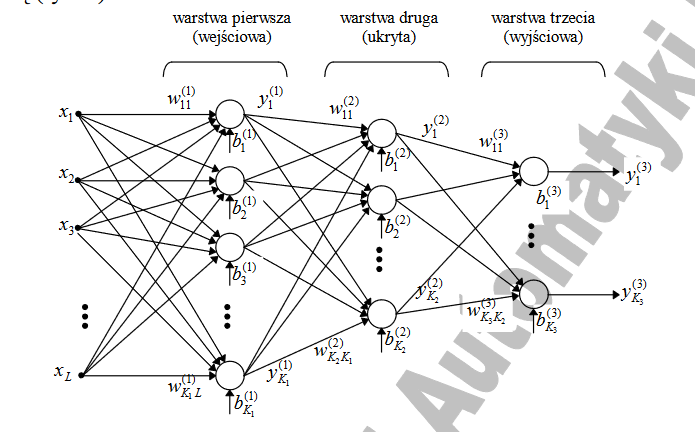
\includegraphics[width=12cm]{figures/models/manyLayerPlaceholder.png}
	\caption{Model prostej sieci trójwarstwowej - Placeholder}
	\label{Fig:multiNetwork}
\end{figure}

W przypadku tego typu sieci ilość macierzy wag jest równa liczbie warstw neuronów.
Oznaczając $y^{(l)}$ jako wyjście, $w^{(l)}$ jako macierz wag, $b^{(l)}$ jako macierz biasów, a $f^{(l)}$ jako funkcję aktywacji neuronów $l-$tej warstwy oraz wykorzystując równanie \ref{eq:singleLayerOut}, w przypadku sieci trójwarstwowej otrzymamy równania:
\begin{equation}
	\label{eq:tripleLayerOut}
	\begin{aligned}
		y^{(1)} &= f^{(1)} \left( w^{(1)} x + b^{(1)} \right)\\
		y^{(2)} &= f^{(2)} \left( w^{(2)} y^{(1)} + b^{(2)} \right)\\
		y^{(3)} &= f^{(3)} \left( w^{(3)} y^{(2)} + b^{(3)} \right)
	\end{aligned}
\end{equation}

Następnie, wykorzystując równania \ref{eq:tripleLayerOut}, możemy opisać działanie całej sieci trójwarstwowej równaniem:

\begin{equation}
	\label{eq:tripleLayerCombined}
	y^{(3)} &= f^{(3)} \left( w^{(3)} f^{(2)} \left( w^{(2)} f^{(1)} \left( w^{(1)} x + b^{(1)} \right) + b^{(2)} \right) + b^{(3)} \right)
\end{equation}

\subsection{Proces uczenia sieci z wykorzystaniem metody gradientowej}
Celem określenia sposobu uczenia sieci, koniecznym jest uprzednie zdefiniowanie tego, co oznacza określenie sieci ,,nauczoną'' bądź ,,nienauczoną''.
W tym celu definiujemy tzw. funkcję kosztu, określającą poziom rozbieżności pomiędzy wartością otrzymaną na wyjściu sieci, a wartością oczekiwaną.
Przykładem takiej funkcji, jest funkcja błędu średniokwadratowego (MSE):
\begin{equation}
	\label{eq:costFunction}
	C\left( w, b, x, a\right) = \frac{1}{2n} \sum\limits_{x} || y\left( x \right) - a ||^2
\end{equation}

W powyższym równaniu, $w$ określa zbiór wszystkich wag wewnątrz sieci, $b$ wszystkich jej biasów, $x$ zbiór danych wejściowych, $n$ ilość danych wejściowych, $y(x)$ zbiór oczekiwanych danych wyjściowych, natomiast $a$ zbiór oczekiwanych wyjść z sieci.
Zakładając, że w procesie uczenia wartości $x$ oraz $a$ pozostają stałe, możemy uprościć oznaczenie funkcji do postaci $C (w,b)$.
Funkcja ta dąży do 0 gdy wartości otrzymywane na wyjściu sieci są bliskie wartościom oczekiwanym, i rośnie wraz ze wzrostem różnicy pomiędzy nimi.
W związku z powyższym, należy znaleźć taką metodę, która pozwoli na minimalizację wartości funkcji $C(w,b)$.

\subsubsection{Ogólny algorytm gradientowy}
Celem zobrazowania problemu rozważmy prostą funkcję $C(v_1, v_2)$ zobrazowaną na rysunku \ref{Fig:simpleCost}.
Naszym celem jest znalezienie jej globalnego minimum.
Teoretycznie możliwe jest jego wyznaczenie metodą analityczną, jednakże według literatury \cite{nndl} jest to rozwiązanie mało wydajne, szczególnie gdy rozważymy funkcje więcej niż kilku zmiennych.

\begin{figure}[ht]
	\centering
	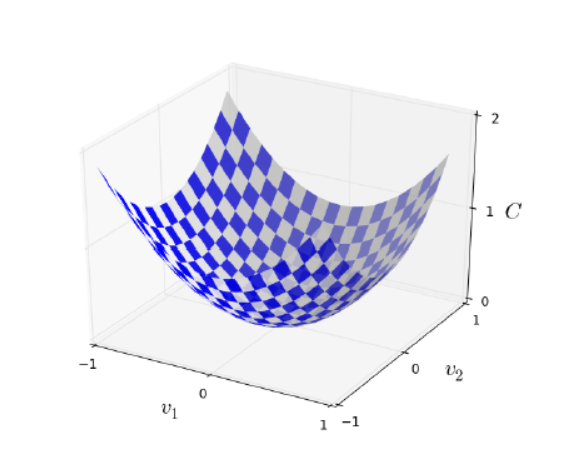
\includegraphics[width=12cm]{figures/models/gradientExample.png}
	\caption{Przykładowa funkcja 2 zmiennych}
	\label{Fig:simpleCost}
\end{figure}

Obserwując rysunek \ref{Fig:simpleCost} możemy jednak dojść do znacznie prostszej obliczeniowo metody.
Przyjmując bliskie zeru wartości $\Delta v_1$ oraz $\Delta v_2$ możemy przyjąć zmianę wartości funkcji $C(v_1, v_2)$ na poziomie:
\begin{equation}
	\label{eq:deltaC}
	\Delta C \approx \frac{\delta C}{\delta v_1} \Delta v_1 + \frac{\delta C}{\delta v_2} \Delta v_2
\end{equation}

Na podstawie powyższego równania możemy zdefiniować wektor zmian:
\begin{equation}
	\label{eq:changeVector}
	\Delta v = (\Delta v_1, \Delta v_2)^T
\end{equation}
oraz tzw. wektor gradientu:
\begin{equation}
	\label{eq:gradientVector}
	\nabla C = \left(\frac{\delta C}{\delta v_1},\frac{\delta C}{\delta v_1}\right)^T
\end{equation}

Wykorzystując powyższe definicje, równanie \ref{eq:gradientVector} możemy zapisać w postaci:
\begin{equation}
	\label{eq:costGradientVector}
	\Delta C \approx \nabla C \cdot \Delta v
\end{equation}

Problemem przy równaniu \ref{eq:costGradientVector} jest wyznaczenie optymalnego wektora $\Delta v$, tak aby zagwarantować ujemną wartość $\Delta C$. W tym celu, możemy przyjąć wartości opisywane równaniem \ref{eq:changeVector} jako równe:
\begin{equation}
	\label{eq:lrNabla}
	\Delta v = -\eta \nabla C
\end{equation}

Wartość $\eta$ nazywana jest ,,współczynnikiem uczenia'' i przyjmuje bliskie zeru, dodatnie wartości. Wykorzystując powyższą definicję, możemy zapisać równanie \ref{eq:costGradientVector} w postaci:
\begin{equation*}
	\begin{aligned}
		\Delta C &\approx - \eta \nabla C \cdot \nabla C\\
		\Delta C &\approx - \eta ||\nabla C||^2
	\end{aligned}
\end{equation*}
W tej postaci równania widzimy, że dla odpowiednio niskiego współczynnika $\eta$ zagwarantowany jest spadek wartości funkcji kosztu $C(v)$.
Wykorzystując właściwość opisaną równaniem \ref{eq:lrNabla} możemy wyznaczyć nowe wartości zmiennych zawartych w wektorze $v$:
\begin{equation}
	\begin{aligned}
		v  \rightarrow v' &= v - \eta \nabla C \\
		v' &= v + \Delta v
	\end{aligned}
\end{equation}

Wielokrotnie aplikując powyższą regułę, jesteśmy w stanie podążać za gradientem aż do osiągnięcia minimum.
Literatura \cite{nndl} definiuje ją jako ,,algorytm spadku gradient'', ale jednocześnie wspomina że w niektórych sytuacjach, może nie być w pełni skuteczna.

\subsubsection{Zastosowanie algorytmu gradientowego w sieciach wielowarstwowych}

Algorytm gradientowy może zostać wykorzystany do minimalizacji funkcji przedstawionej równaniem \ref{eq:deltaC}, poprzez odnajdowanie wartości wag oraz biasów minimalizujących funkcję kosztu.
Wykorzystując oznaczenia $w^{(l)}_{ij}$ jako j-tą wagę i-tego neuronu l-tej warstwy oraz $b^{(l)}_i$ jako bias i-tego neuronu w l-tej warstwie, możemy wyznaczyć ich wartości w kolejnych iteracjach (epokach) procesu uczenia:
\begin{equation}
	\label{eq:weightUpdate}
	w^{(l)}_{ij} \rightarrow {w'}^{(l)}_{ij} = w^{(l)}_{ij} - \eta \frac{\delta C}{\delta w^{(l)}_{ij}}
\end{equation}
\begin{equation}
	\label{eq:biasUpdate}
	b^{(l)}_{i} \rightarrow {b'}^{(l)}_{i} = b^{(l)}_{i} - \eta \frac{\delta C}{\delta b^{(l)}_{i}}
\end{equation}

Przyjmując jako funkcję kosztu błąd średniokwadratowy, przy założeniu wystąpienia wielu danych uczących, możemy ją zapisać w postaci:
\begin{equation}
	C = \frac{1}{n} \sum \limits_x C_x
\end{equation}
czyli średniej wartości błędów $C_{x} = \frac{||y(x) - a||^2}{2}$ dla poszczególnych par uczących.

TODO: Rozpisać wzory na poszczególne pochodne - instrukcja \cite{kiaMultiLayer}



\subsubsection{Metoda stochastycznego spadku gradientu}
Jednym z problemów algorytmu spadku gradientu, objawiającym się przy dużej liczbie rekordów uczących \cite{nndl} jest długi czas potrzebny na obliczanie wartości pochodnych w równaniu \ref{eq:gradientVector}.
Celem zniwelowania tego problemu można wykorzystać metodę zwaną ,,stochastycznym spadkiem gradientu''.
Polega ona na oszacowaniu rzeczywistego gradientu $\nabla C$ poprzez obliczenie $\nabla C_x$ dla losowo wybranej próbki danych uczących.
Poprzez odpowiednie dobranie rozmiaru próbek, oraz ich odpowiednie uśrednienie, możemy uzyskać dobre przybliżenie rzeczywistego gradientu $\nabla C$.\cite{nndl}
Elementy pojedynczej próbki możemy oznaczyć jako $X_1, X_2, \ldots , X_m$
Zakładając odpowiednio duży rozmiar $m$ możemy przyjąć za prawdziwe równanie:
\begin{equation}
	\label{eq:stochasticGradient}
	\frac{ \sum_{j=1}^{m} \nabla C_{X_j}}{m} \approx \frac{ \sum_x \nabla C_x}{n} = \nabla C
\end{equation}

Przenosząc czynnik $\frac{1}{m}$ przed znak sumy, otrzymamy:
\begin{equation}
	\label{eq:stochasticGradientFinal}
	\nabla C \approx \frac{1}{m} \sum_{j=1}^{m} \nabla C_{X_j}
\end{equation}

Wartym zauważenia jest też fakt występowania różnych konwencji uśredniania czy też skalowania gradientu stochastycznego. \cite{nndl}
Niektóre źródła mówią o braku konieczności ich stosowania gdyż wpływają na działanie sieci jedynie pośrednio, poprzez modyfikację wartości współczynnika uczenia.
Z tego też powodu, w dalszej implementacji przyjęto współczynnik równy stosunkowi rozmiaru próbki do rozmiaru całego zbioru uczącego.

\subsubsection{Adaptacyjny współczynnik uczenia}
W równaniu \ref{eq:lrNabla} wprowadzono pojęcie współczynnika uczenia.
Standardowa metoda gradientowa zakłada że jest on stały przez cały okres uczenia sieci, a jego odpowiedni dobór jest jednym z kryteriów koniecznych do poprawnego przebiegu procesu uczenia.
Nie jest to jednak rozwiązanie optymalne, gdyż zbyt duża jego wartość może znacząco utrudnić osiągnięcie minimum funkcji błędu a w skrajnych przypadkach spowodować rozbiegnięcie procesu uczenia.
Zbyt mała jego wartość również jest niekorzystna gdyż znacznie wydłuża czas potrzebny na osiągnięcie celu uczenia - definiowanego jako minimalizacja funkcji wyrażonej równaniem \ref{eq:costFunction}.

Jedną z metod pozwalających zniwelować ten problem, jest metoda adaptacyjnej korekty współczynnika uczenia $\eta $\cite{kiaAcc}.
Przyjmując wartość błędu w chwili czasu $t$:
\begin{equation}
	\label{eq:costFunctionTimed}
	MSE(t) = \frac{1}{2n} \sum_{i=1}^{M}  || y_{i}(t) - a(t) ||^2
\end{equation}
Możemy zdefiniować sposób korekty współczynnika uczenia jako:
\begin{equation}
	\label{eq:adaptiveLR}
	\eta \left( t + 1 \right)  =
	\begin{cases}
		\eta \left( t \right) \cdot \xi_d & \text{gdy } MSE(t) > er \cdot MSE(t-1)\\
		\eta \left( t \right) \cdot \xi_i & \text{gdy } MSE(t) <  MSE(t-1)\\
		\eta \left( t \right)  & \text{gdy } MSE(t-1) \leq MSE(t) \leq er \cdot MSE(t-1)
	\end{cases}
\end{equation}
gdzie $\xi_d$ $\xi_i$ są odpowiednio współczynnikami zmniejszania i zwiększania wartości współczynnika uczenia, zaś $er$ określa dopuszczalną krotność przyrostu błędu.
Podejście takie powoduje wprawdzie konieczność ustalenia dodatkowych parametrów w procesie uczenia, lecz eliminuje problem doboru współczynnika uczenia.
Jeśli będzie on zbyt duży, zostanie zredukowany do pożądanego poziomu ze względu na wzrastający poziom błedu.
Jednocześnie zbyt niska wartość $\eta$ zostanie zwiększona kiedy proces uczenia natrafi na bardziej optymalne warunki.

Literatura \cite{nnd} podaje także bardziej skomplikowany wariant zastosowania zmiennego współczynnika uczenia.
Polega on na dodatkowym zapisywaniu stanu wag oraz biasów przed ich zmianą wynikającą z algorymtu spadku gradientu.
Wagi te mogą następnie zostać przywrócone jeśli uczenie przyniosło efekt odwrotny do zamierzonego i doszło do wzrostu wartości błędu.
W praktyce oznacza to przywrócenie zachowanych wag oraz biasów w momencie zmniejszenia $\eta$ o współczynnik \xi_d.

\section{Implementacja algorytmów w języku Rust}
Przed wykonaniem badań operujących na przedstawionych algorytmach, konieczna była ich implementacja w postaci pozwalającej na proste ustalanie parametrów sieci, oraz jej ewentualne modyfikacje na potrzeby eksperymentów.
W tym celu wykorzystany został język programowania ogólnego przeznaczenia - Rust, oraz następujące biblioteki:
\begin{itemize}
	\item ndarray 0.15.4 - wykorzystywana do obliczeń związanych z algebrą liniową, przede wszystkim operacji na macierzach
	\item rand 0.8.5 - wykorzystywana do generowania liczb losowych
\end{itemize}
Pełny kod gotowy do kompilacji i uruchomienia znajduje się na repozytorium: \url{https://github.com/MatiF100/AI_Project}.

\subsection{Implementacja struktury sieci}
\subsubsection{Podstawowa struktura reprezentująca sieć}
Pierwszym krokiem koniecznym do realizacji projektu było wykonanie ogólnej struktury sieci, pozwalającej na ustalenie jej parametrów, oraz funkcji pozwalającej na jej inicjalizację.


\begin{lstlisting}[language=Rust,caption=Podstawowa struktura sieci neuronowej,label={lst:netStructure}]
#[derive(Debug, Clone)]
struct Network {
    layers: Vec<usize>,
    biases: Vec<Array2<f64>>,
    weights: Vec<Array2<f64>>,
    name: String,
}
\end{lstlisting}

\begin{lstlisting}[language=Rust,caption=Konstruktor struktury sieci neuronowej,label={lst:netConstructor}]
fn new(layers: Vec<usize>) -> Self {
	let mut rng = rand::thread_rng();
	let layers = layers
		.into_iter()
		.filter(|x| *x > 0)
		.collect::<Vec<usize>>();
	Self {
		name: String::from("Network 0"),
		//Biases are initialized with random values
		biases: layers
			.iter()
			.skip(1)
			.map(|&s| {
				(0..s)
					.map(|_| rng.gen_range::<f64, std::ops::Range<f64>>(-1.0..1.0))
					.collect::<Vec<f64>>()
			})
			.map(|v| Array2::from_shape_vec((v.len(), 1), v).unwrap())
			.collect(),

		//Weights are also initialized with random values
		weights: layers
			.windows(2)
			.map(|x| {
				(
					(x[0], x[1]),
					(0..x[0] * x[1])
						.map(|_| rng.gen_range::<f64, std::ops::Range<f64>>(-1.0..1.0))
						.collect::<Vec<f64>>(),
				)
			})
			.map(|(x, v)| Array2::from_shape_vec((x.1, x.0), v).unwrap())
			.collect::<Vec<_>>(),
		//Layers are moved in from the argument
		layers,
	}
}

\end{lstlisting}

Sieć została zbudowana w sposób dający dużą swobodę w ustalaniu jej parametrów - zarówno liczba warstw jak i neuronów w poszczególnych warstwach może być łatwo modyfikowana przez podanie odpowiedniego wektora jako argumentu.


\begin{lstlisting}[language=Rust,caption=Utworzenie przykładowej struktury sieci,label={lst:netExample}]
fn main(){
	let (R, S1, S2, S3) = (16, 8, 6, 2);
	let x = Network::new(vec![R, S1, S2, S3]);
}
\end{lstlisting}

Powyższy kod tworzy sieć neuronową o 16 wejściach, 8 neuronach w warstwie 1, 6 neuronach w warstwie drugiej oraz 2 neuronach w warstwie trzeciej.
Dla uproszczenia kodu i przyspieszenia obliczeń, wejścia sieci są reprezentowane jako dodatkowa warstwa neuronów, których wyjście w trakcie działania sieci jest ustalane do wartości znajdujących się w wektorze wejściowym.
Również dla uproszczenia kodu, przyjęto stałą funkcję aktywacji dla każdego z neuronów, opisaną równaniem \ref{eq:sigmoid}.


\begin{lstlisting}[language=Rust,caption=Funkcja sigmoidalna oraz jej pochodna,label={lst:sigmoid}]
//Sigmoidal function - basic activation function for neurons
fn sigmoid<D>(z: Array<f64, D>) -> Array<f64, D>
where
    D: Dimension,
{
    let mut z = z;
    z.iter_mut().for_each(|f| *f = 1.0 / (1.0 + (-*f).exp()));
    z
}

//Derivative of sigmoidal function
fn sigmoid_prime<D>(z: Array<f64, D>) -> Array<f64, D>
where
    D: Dimension,
{
    let val = sigmoid(z);
    &val * (1.0 - &val)
}
\end{lstlisting}

Powyższa implementacja nie jest optymalna, gdyż zakłada obliczanie wartości funkcji aktywacji przy każdym wywołaniu funkcji zwracającej jej pochodną, podczas gdy zwykle wartość ta była już obliczona wcześniej.
Możliwe jest zatem dalsza optymalizacja kodu, co jednakże nie jest konieczne dla przeprowadzenia większości eksperymentów.


\begin{lstlisting}[language=Rust,caption=Realizacja funkcji feed-forward,label={lst:sigmoid}]
fn feed_forward(&self, mut a: Array2<f64>) -> Array2<f64> {
	for (b, w) in self.biases.iter().zip(self.weights.iter()) {
		a = sigmoid(w.dot(&a) + b);
	}
	return a;
}
\end{lstlisting}

Ostatnią funkcją konieczną do działania sieci jest funkcja feedforward, pobierająca dane z wejścia sieci, i zwracająca wynikowy wektor stopnia aktywacji neuronów wyjściowych.

\subsubsection{Algorytm uczenia sieci}
\begin{lstlisting}[language=Rust,caption=Realizacja funkcji stochastycznego spadku gradientu,label={lst:sgd}]
 fn sgd(
	&mut self,
	training_data: &mut Vec<(Array2<f64>, Array2<f64>)>,
	epochs: usize,
	mini_batch_size: usize,
	mut eta: f64,
	test_data: Option<&Vec<(Array2<f64>, usize)>>,
	eta_mod: Option<(f64, f64)>,
	target_cost: f64,
	report_interval: usize,
) {
	let mut rng = rand::thread_rng();

	//Main loop performing learning step with each epoch
	for j in 1..=epochs {
		//Randomization of data for usage of mini-batch
		training_data.shuffle(&mut rng);

		//Generation of mini-batch vector. This is basicaly a collection of smaller datasets
		let mut mini_batches = training_data
			.windows(mini_batch_size)
			.step_by(mini_batch_size)
			.map(|s| s.to_vec())
			.collect::<Vec<Vec<_>>>();

		let batch_count = mini_batches.len();
		// Branching based on existance of adaptive learning rate parameters
		match eta_mod {
			Some((dec, inc)) => {
				// Saving state of network before readjustment of weights and biases
				let saved_weights = self.weights.clone();
				let saved_biases = self.biases.clone();
				let previous_error = self.mse(training_data);

				//Sub-loob performing learning step for each of the mini-batch
				for mini_batch in &mut mini_batches {
					//dbg!(&mini_batch);
					self.update_mini_batch(mini_batch, eta, batch_count)
				}

				// Verification of newly achieved Mean Square Error
				let new_error = self.mse(training_data);
				if new_error < target_cost {
					if let Some(data) = &test_data {
						let output = self.evaluate(data);
						println!("{},{}", self.name, output.1 as f64 / output.0 as f64);
					}
					break;
				}
				if new_error > previous_error * MAX_PERF_INC {
					// Restoring backup
					self.weights = saved_weights;
					self.biases = saved_biases;

					// Adaptation - learning rate decreases
					eta *= dec;
				} else if new_error < previous_error {
					// Adaptation - learning rate increases
					eta *= inc;
				}
				// else statement does nothing - ommited
			}
			None => {
				//Sub-loob performing learning step for each of the mini-batch
				for mini_batch in &mut mini_batches {
					//dbg!(&mini_batch);
					self.update_mini_batch(mini_batch, eta, batch_count);
					let new_error = self.mse(training_data);
					if new_error < target_cost {
						if let Some(data) = &test_data {
							let output = self.evaluate(data);
							println!("{},{}", self.name, output.1 as f64 / output.0 as f64);
						}
						break;
					}
				}
			}
		}

		//Data verification. Can be ommited
		if let Some(data) = &test_data {
			if j + 1 % report_interval == 0 && report_interval != 0 {
				let output = self.evaluate(data);
				println!("{},{}", self.name, output.1 as f64 / output.0 as f64);
			}
		} else {
			//println!("Epoch {} complete!", j);
		}
	}
}
\end{lstlisting}

Powyższy kod realizuje uogólniony przypadek funkcji spadku gradientu.
W jego ramach można wyróżnić kilka bloków funkcjonalnych.
Pierwszym z nich jest definicja funkcji spadku gradientu oraz jej parametrów:
\begin{itemize}
	\item &mut self - mutowalna referencja do struktury Network, słowo kluczowe self oznacza że funkcja stanowi metodę struktury Network
	\item training\_data - mutowalna referencja do wektora przechowującego pary uczące
	\item epochs - maksymalna liczba epok przez które należy wykonywać algorytm
	\item mini\_batch\_size - rozmiar próbki w metodzie stochastycznej (ustawiona na wartość równą długości wektora training\_data będzie równoważne z brakiem podziału danych uczących)
	\item mut eta - mutowalna wartość zmiennoprzecinkowa, współczynnik uczenia
	\item test\_data - opcjonalna referencja do wektora przechowującego dane wykorzystywane do walidacji krzyżowej
	\item eta\_mod - opcjonalne parametry wykorzystywane w ramach adaptacyjnego współczynnika uczenia
	\item target\_cost - docelowy błąd
	\item report\_interval - liczba epok co którą sieć wykonuje walidację krzyżową i wyświetla raport
\end{itemize}

Następnym etapem, działającym już wewnątrz pętli jest wykonanie  podziału zbioru uczącego na mniejsze próbki (o ile następuje taka konieczność).
Dalsza część funkcji opiera się na opcjonalnym parametrze eta\_mod.
Jeśli jest on obecny, wykonywany jest algorytm powiązany z adaptacyjnym współczynnikiem uczenia.
W każdej iteracji pętli, parametry sieci oraz poprzedni błąd są zapisywane przed wykonaniem operacji uczenia, a następnie w zależności od uzyskanego wyniku, wykonywana jest jedna z operacji opisana w równaniu \ref{eq:adaptiveLR}.
Jeżeli natomiast nie podano parametrów modyfikacji współczynnika uczenia, wykonywany jest klasyczny algorytm bez przyspieszeń.
W trakcie uczenia, wykorzystywana jest funkcja update\_mini\_batch(...), którą przedstawiono na listingu \ref{lst:updateMB}.

Ostatnim elementem pętli jest natomiast walidacja krzyżowa.
Zachodzi jeśli podano zostały podane dane weryfikacyjne, a numer obecnej epoki jest wielokrotnością zadanego interwału raportu.
Działanie algorytmu walidacji krzyżowej prezentuje listing \ref{lst:eval}

\begin{lstlisting}[language=Rust,caption=Realizacja funkcji walidacji krzyżowej,label={lst:eval}]
fn evaluate(&self, test_data: &Vec<(Array2<f64>, usize)>) -> (usize, usize) {
	let mut local_data = test_data.clone();
	let x = local_data
		.iter_mut()
		.map(|(x, y)| {
			(
				self.feed_forward(x.clone())
					.iter()
					.enumerate()
					.max_by(|(_, a), (_, b)| {
						a.partial_cmp(b).unwrap_or(std::cmp::Ordering::Equal)
					})
					.map(|(index, _)| index),
				y,
			)
		})
		.filter(|(a, b)| a.unwrap_or(0) == **b)
		.count();
	(test_data.len(), x)
}
\end{lstlisting}
Ponieważ w przyjętej implementacji sieci neuronowej, każdy z neuronów posiada sigmoidalną funkcję aktywacji, konieczne jest zdefiniowanie jednoznacznego sposobu określenia, do jakiej klasy sieć przypisuje obiekt o zadanych parametrach.
Powyższa implementacja zakłada w tym celu wykorzystanie n neuronów wyjściowych, gdzie n oznacza liczbę istniejących klas.
Określenie wyniku klasyfikacji odbywa się poprzez funkcję maksimum, zwracającą indeks neuronu wyjściowego o najwyższym stopniu aktywacji.
Warto zaznaczyć że w powyższej implementacji nie jest istotna sama wartość aktywacji neuronu, a jedynie jej stosunek względem pozostałych neuronów warstwy wyjściowej.


\begin{lstlisting}[language=Rust,caption=Realizacja funkcji update\_mini\_batch,label={lst:updateMB}]
fn update_mini_batch(
	&mut self,
	mini_batch: &Vec<(Array2<f64>, Array2<f64>)>,
	eta: f64,
	batches_count: usize,
) {
	// Allocation of gradient vectors
	let mut nabla_b = self
		.biases
		.iter()
		.map(|b| Array::zeros(b.raw_dim()))
		.collect::<Vec<Array2<f64>>>();
	let mut nabla_w = self
		.weights
		.iter()
		.map(|w| Array::zeros(w.raw_dim()))
		.collect::<Vec<Array2<f64>>>();

	// Loop performing learning iteration over all mini_batches
	for (x, y) in mini_batch {
		// Getting updated gradients from backpropagation algorithm
		let (delta_nabla_b, delta_nabla_w) = self.backprop(x, y);

		// Calculating new gradients with respect to ones created in first steps and also newly calculated ones
		nabla_b = nabla_b
			.iter()
			.zip(delta_nabla_b.iter())
			.map(|(nb, dnb)| nb + dnb)
			.collect();
		nabla_w = nabla_w
			.iter()
			.zip(delta_nabla_w.iter())
			.map(|(nw, dnw)| nw + dnw)
			.collect();
	}

	// Calculating new values for weights and biases based on recieved gradients with respect to batch size and learning rate
	self.weights = self
		.weights
		.iter()
		.zip(nabla_w.iter())
		.map(|(w, nw)| w - nw * (eta / batches_count as f64) as f64)
		.collect();
	self.biases = self
		.biases
		.iter()
		.zip(nabla_b.iter())
		.map(|(b, nb)| b - nb * (eta / batches_count as f64) as f64)
		.collect();
}
\end{lstlisting}
Powyższa funkcja oblicza wartości gradientów dla wyodrębnionych w poprzednim etapie algorytmu próbek.
Parametry przyjmowane przez funkcję to:
\begin{itemize}
	\item &mut self - mutowalna referencja do struktury Newtork
	\item mini\_batch - referencja do próbki danych uczących
	\item eta - współczynnik uczenia
	\item batches\_count - liczba wszystkich próbek wyodrębnionych z danych uczących
\end{itemize}

Funkcja ta alokuje bufor o stałym rozmiarze, a następnie używa go do sumowania gradientów obliczanych dla poszczególnych par uczących w funkcji backprop(...) opisanej listingiem \ref{lst:backprop}.
Następnie na podstawie obliczonego gradientu wykonywana jest aktualizacja wag. Procedurę realizowaną przez tą funkcję opisują równania \ref{eq:weightUpdate} oraz \ref{eq:biasUpdate}.

\begin{lstlisting}[language=Rust,caption=Realizacja funkcji wstecznej propagacji błędu,label={lst:backprop}]
fn backprop(&self, x: &Array2<f64>, y: &Array2<f64>) -> (Vec<Array2<f64>>, Vec<Array2<f64>>) {
	//Initialization of gradient vectors.
	let mut nabla_b = self
		.biases
		.iter()
		.map(|b| Array::zeros(b.raw_dim()))
		.collect::<Vec<Array2<f64>>>();
	let mut nabla_w = self
		.weights
		.iter()
		.map(|w| Array::zeros(w.raw_dim()))
		.collect::<Vec<Array2<f64>>>();

	// Preparing initial information for forward network pass
	// Because of lifetimes and loop scope further in the function, it is best to make copies of input matrix here
	let mut activation = x.clone();
	let mut activations = vec![activation];

	// zs is a Vector of neurons non linear blocks inputs - these will be calculated in the following loop
	let mut zs: Vec<Array2<f64>> = Vec::new();

	// Performing feedforward operation
	for (b, w) in self.biases.iter().zip(self.weights.iter()) {
		// z is the input of non-linear block, necessary in the following gradient calculation
		let z = w.dot(activations.iter().last().unwrap()) + b;
		zs.push(z.clone());

		// As the current matrix of non-linear block inputs is calculated, it is passed as argument to the activation function
		// TODO: in this place other activation functions can be implemented
		activation = sigmoid(z);

		// Saving the outputs of neuron layer, for later use
		activations.push(activation);
	}

	// Calculating per_class or per_output cost of the result at this point, it is also worth noting that the "delta" is only partially calculated
	// With used notation, the delta itself does not include the eta, or learning rate
	// Cost derivative function only calculates error, or difference between achieved and expected output
	// TODO: possibly unnecessary function call
	let mut delta = Self::cost_derivative(activations.last().unwrap().clone(), y.clone())
		* sigmoid_prime(zs.last().unwrap().clone());

	// Setting up known values in gradient vectors
	// Last layer is easiest to calculate, as it does not require any data not available at the moment
	// We they will be used as we perform the backward pass, calculating bias and weight gradients for every layer
	*nabla_b.last_mut().unwrap() = delta.clone();
	*nabla_w.last_mut().unwrap() = delta.dot(&activations[activations.len() - 2].t());

	// Performing backward network pass
	// Side note: if the book gives example of any identifier as "l" "I" or "L" one should never follow the book and come up with anything that differs from 1
	for idx in 2..self.layers.len() {
		// Getting the input of non-linear block for the idx-th layer counting from the end
		let z = &zs[zs.len() - idx];

		// Calculating the derivative of activation function for given input
		let derivative = sigmoid_prime(z.clone());

		// Calculating delta - gradient for given layer
		// TODO: Include the generic formula into readme
		delta = self.weights[self.weights.len() - idx + 1].t().dot(&delta) * derivative;

		// Boilerplate forced by borrow-checker. Since .len() uses immutable reference, it would block the assignment operation if used inline
		// Works fine this way though, since usize implements "Copy"
		let b_len = nabla_b.len();
		let w_len = nabla_w.len();

		// Actual gradient for biases and weights is pretty similar
		// The difference is that weight gradient is additionally multiplied by the activation state of given layer
		nabla_b[b_len - idx] = delta.clone();
		nabla_w[w_len - idx] = delta.dot(&activations[activations.len() - idx - 1].t());
	}

	// Returning calculated gradient vectors
	(nabla_b, nabla_w)
}

fn cost_derivative(output_activations: Array2<f64>, y: Array2<f64>) -> Array2<f64> {
	output_activations - y
}
\end{lstlisting}

Argumentami powyższej funkcji backprop(...) są kolejno:
\begin{itemize}
	\item &self - referencja do struktury Network
	\item x - wektor parametrów pary uczącej
	\item y - oczekiwane wyjście dla zadanych parametrów
\end{itemize}
Dodatkowo zdefiniowana została funkcja pomocnicza cost\_derivative(...) zwracająca wektor pochodnych funkcji błędu dla każdego z wyjść, względem wyjść neuronów warstwy wyjściowej.
Dla przyjętej funkcji błędu przyjmuje ona postać różnicy pomiędzy wyjściem sieci, a wyjściem oczekiwanym.


W pierwszej kolejności, podobnie jak w funkcji \ref{lst:updateMB} alokowana jest pamięć potrzebna na przechowanie obliczonych gradientów.
Następnie zostają przygotowane zmienne przechowujące wartości wyjścia (aktywacji) neuronów oraz wejścia funkcji aktywacji.
Kolejnym krokiem jest obliczenie oraz zachowanie wartości wejść oraz wyjść funkcji aktywacji neuronów w poszczególnych warstwach.
Po wykonaniu pętli, obliczana jest wartość delta, a na jej podstawie wartości gradientów dla ostatniej warstwy wag oraz biasów.
W ostatnim kroku, ponownie wykonywana jest pętla, która powtarza poprzedni krok dla pozostałych warstw, obliczając wartości gradientów dla warstw od przedostatniej do pierwszej (wejściowej).
Obliczone w ten sposób wektory gradientów są następnie zwracane z funkcji.



\section{Wstęp/wprowadzenie}
1 $\div$ 5 stron charakterystyka problematyki w świetle aktualnego stanu wiedzy i~techniki, ze wskazaniem na zagadnienia istotne z punktu widzenia realizowanej pracy.
Na trzeciej stronie można zamieścić podziękowania dla osób, które przyczyniły się do powstania pracy dyplomowej. Na kolejnej stronie nieparzystej rozpoczyna się spis treści. Po spisie treści zalecane jest umieszczenie wykazu użytych symboli, oznaczeń i akronimów. Od tego miejsca rozpoczyna się numeracja rozdziałów. Na następnej stronie umieszcza się wprowadzenie do pracy (scharakteryzowanie problematyki pracy, uzasadnienie wyboru tematyki) oraz przedstawia: cel i/lub tezę pracy, zakres pracy, przyjęte założenia itp.
Ostatni akapit wstępu musi zawierać zwięzłe sformułowanie celu i zakresu pracy. 
\\
\textcolor{red}{
Uwaga: \\
Jeżeli decydujesz się wykorzystywać \LaTeX'a, ignoruj ogólny dokument dotyczący formatowania pracy dyplomowej na WEiI - jest przeznaczony dla użytkowników innych edytorów tekstu. Korzystaj z załączonego arkusza stylu, stosuj formatowanie znaczeniowe (nie wymuszaj formatowania), a wynikowa praca będzie zgodna z wymaganiami. Zachęcamy do używania \LaTeX'a, czas poświęcony na jego przyswojenie, zwróci się z nawiązką nawet w trakcie tworzenia pracy dyplomowej. \\
Niniejszy tekst, wykorzystujący  styl \texttt{weiiszablon.sty} zawiera informacje o formatowaniu, wielkości czcionek, wyrównania\ldots, ale \textbf{uwaga}, sama treść nie jest istotna (np. opis wielkości czcionek), 
formatowanie wykona się automatycznie, tu te zapisy są tylko po to, aby dostarczyć dokument zawierający jak najwięcej przykładów użycia \LaTeX'a.
}

\clearpage

\section{Tekst zasadniczy -- I}

Do 20\% objętości pracy. W zależności od charakteru pracy ten rozdział powinien zawierać:
\begin{enumerate}[label=\alph*), leftmargin=1.25cm]
	\item opis tematyki zagadnienia -- aktualny stan zagadnienia,
	\item metody i rozwiązania,
	\item dyskusja i krytyczna ocena stanu aktualnego,
	\item podsumowanie stanu wiedzy, techniki literaturowe itp.
\end{enumerate}

\subsection{Formatowanie rozdziałów i podrozdziałów}
Rozdziały zaczynają się u góry nowej strony (parzystej lub nieparzystej). Podrozdziały i zakresy mogą zaczynać się w dowolnym miejscu strony. Przy końcu pracy zamieszcza się podsumowanie i wnioski. Ostatni akapit podsumowania musi zawierać wyszczególnienie własnej pracy Autora i zaczynać się od sformułowania: „Autor za własny wkład pracy uważa:”. W tym miejscu kończy się numeracja rozdziałów.

Ewentualne listingi programów, instrukcje obsługi stanowisk lub inne tego rodzaju materiały zaleca się zamieścić w formie dodatków. Kolejno zamieszcza się: wykaz literatury, spis rysunków/tabel oraz streszczenie (zgodne ze „Wzorem streszczenia”). Wykaz literatury rozpoczyna od strony nieparzystej.

Opisując własne dokonania, stosuje się formę bezosobową w czasie przeszłym np. celem pracy było zaprojektowanie\ldots, zakres pracy obejmował wyznaczenie\ldots, w~ramach pracy wykonano model\ldots itp.
\clearpage	

\section{Tekst zasadniczy -- II}

Ponad 50\% objętości pracy -- część autorska:
\begin{enumerate}[label=\alph*), leftmargin=1.25cm] 
	\item założenia – dane,
	\item opis zastosowanej metody rozwiązania lub analizy,
	\item opis proponowanego rozwiązania, wyniki analizy teoretycznej, obliczenia, projekt konstrukcyjny, procesowy, technologiczny,
	\item wyniki badań analitycznych, symulacyjnych lub eksperymentalnych itp.
\end{enumerate}

Przy stosowaniu podziału na rozdziały i podrozdziały zaleca się unikać podziału więcej niż trzystopniowego. Podział tekstu, szczególnie na rozdziały główne, wynikać powinien z zakresu i charakterystyki realizowanej pracy.

\subsection{Formatowanie tekstu. Należy pamiętać, że na końcu tytułu rozdziału, podrozdziału i zakresu nie umieszcza się kropki}

\subsubsection{Marginesy i akapity}

Marginesy deklaruje się jako „lustrzane” i ustawia na 2 cm, na oprawę 1,5 cm. 
Nagłówek i stopka 1,25 cm. Tekst podstawowy akapitu: czcionka szeryfowa, styl Times (Times New Roman, Liberation Serif itp.), rozmiar 12 punktów, interlinia 1,5 wiersza. Akapit wyjustowany, wcięcie pierwszego wiersza 1,25 cm. 

Na końcu każdego akapitu, którego tekst zaczerpnięto z literatury, musi znajdować się odnośnik do właściwej pozycji w wykazie literatury. W pracy nie stosuje się
odnośników w formie przypisów. Liczby w nawiasie kwadratowym oznaczają kolejny numer pozycji w wykazie, np. [1] lub [1, 4, 7] lub [1, 6-8] itp.

Cytaty (dosłowne przytoczenie obcego tekstu w pracy) pisze się czcionką pochyłą (kursywą) i ujmuje w cudzysłów. Przykład: „\textit{Współpracując z jednostkami gospodarczymi działającymi w kraju, kształci wysokokwalifikowaną kadrę inżynierów}”.

Fragmenty kodów programów pisze się czcionką o stałej szerokości, styl \footnotesize {\texttt{Courier}}
\normalsize{(Courier New, Liberation Mono itp.) o rozmiarze 10 punktów.}


\subsubsection{Zalecenia co do sposobu pisania jednostek i symboli wielkości fizycznych}

Poniższy podrozdział opracowano na podstawie \cite{Pawluk2001}. W trakcie pisania pracy należy zwracać uwagę na sposób oznaczania jednostek i symboli wielkości fizycznych. Przy zapisywaniu jednostek i symboli wielkości fizycznych można wyróżnić zapis w~postaci kursywy (pismo pochyłe) oraz antykwy (pismo proste). 

\begin{enumerate}[label=\arabic*), leftmargin=1.25cm]
\item Kursywę należy stosować w następujących przypadkach:

\begin{itemize}[label=-,labelsep=0.4cm,leftmargin=0.6cm] %[leftmargin=0.65cm]
\item symboli wielkości fizycznych niezależnie od tego czy jest to litera alfabetu greckiego (np. przenikalność magnetyczna $\mu$) czy też łacińskiego (np. rezystancja $R$). Należy przestrzegać tej zasady niezależnie od miejsca, w którym pojawia się symbol tj. tekst, wzory matematyczne, rysunki, tabele,

\item ogólny symbol zapisu funkcji czyli np. $f$, a nie f. Nie dotyczy to jednak zapisu konkretnych funkcji np. $\cos \omega t$ a nie $cos \omega t$,

\item macierze, wektory, których elementami są wielkości fizyczne należy zapisywać dodatkowo czcionką półgrubą (bold) np. 
$\bm{R} = \left[ 
\begin{array}{cc}
R_{11} & R_{12} \\
R_{21} & R_{22} 
\end{array} 
\right]$,
$\bm{U} = \left[ 
\begin{array}{c}
U_{1} \\
U_{2} 
\end{array} 
\right]$,

\item wskaźnik dolny, górny, prawo- i lewostronny, ale tylko gdy odnosi się do konkretnej wielkości fizycznej, czyli np. składowa $x$-owa indukcji magnetycznej $B_x$, a nie $B_{\mathrm{x}}$,

\item wskaźniki górne i dolne oznaczające dowolną liczbę np. $R_j$, $I^k$, ale nie $R_\mathit{1}$, $I^\mathit{2}$.

\end{itemize}

\item Antykwę należy stosować w następujących sytuacjach:

\begin{itemize}[label=-,labelsep=0.4cm,leftmargin=0.6cm]
\item wszystkie cyfry,

\item symbole konkretnych funkcji np. $\mathrm{tg\ } \omega t$, a nie $tg \omega t$,

\item operatory operacji matematycznych np. pochodne zwyczajne $\frac{\mathrm{d} x}{\mathrm{d} t}$, a nie $\frac{d x}{d t}$,

\item symbole liczb o konkretnej wartości np. przenikalność elektryczna próżni $\varepsilon_0 = 8,8542 \cdot 10^{-12}$ $\mathrm{F} \cdot \mathrm{m}^{-1}$, a nie $\varepsilon_0 = 8,8542 \cdot 10^{-12}$ $\mathrm{F} \cdot \mathrm{m}^{-1}$,

\item indeksy, jeżeli odnoszą się do: obiektów (fizycznych, geometrycznych), czyli, np. natężenie pola elektrycznego w punkcie A to $E_\mathrm{A}$, a nie $E_A$, zjawisk lub stanów fizycznych, np. moment obciążenia to $T_\mathrm{L}$, a nie $T_L$, do nazwisk czy też oznaczeń pierwiastków, np. straty w miedzi to $P_{\mathrm{Cu}}$ a nie $P_{Cu}$, do charakteru wielkości symbolizowanej przez literę źródłową, np. wartość maksymalna siły to $F_\mathrm{max}$, a nie $F_{max}$, oznaczeń jednostek miary np. $\mathrm{M}\Omega$, a nie $M \mathit{\Omega}$.

\end{itemize}

\item W przypadku jednostek miar (które zawsze należy pisać antykwą) zapisując konkretną wartość liczbą należy podać jej wartość i jednostkę z zachowaniem następujących zasad:

\begin{itemize}[label=-,labelsep=0.4cm,leftmargin=0.6cm]
\item zapisując wartość liczbową wielkości fizycznej po spacji należy podać jej jednostkę, ale nie nazwę jednostki np. $10 \mathrm{A}$, ale nie $10$ amper czy też $10$ amperów,

\item zapisując wartość liczbową słownie należy w tej konwencji podać też jednostkę np. dziesięć omów, ale nie dziesięć $\Omega$

\item do oznaczeń jednostek nie wolno dopisywać indeksów, np. moc wyjściowa silnika wynosi $P=100$ $\mathrm{kW}_\mathrm{out}$. W takim przypadku należy zapisać $P_\mathrm{out}=100$ $\mathrm{kW}$,

\item jednostek nie należy umieszczać w nawiasach kwadratowych, np. $I=1$ $\mathrm{[A]}$. Odstępstwem od tej zasady mogą być tabele, nagłówki kolumn, opisy osi na wykresach oraz w sporadycznych sytuacjach we wzorach matematycznych (ale tylko wówczas, gdy zależność matematyczna nie wskazuje w~jakiej jednostce wystąpi wartość liczbowa). Przykłady odstępstw zamieszczono w~podrozdziale \ref{Subsec:Rysunki-i-tabele}.   

\end{itemize}

\item W trakcie zapisu symboli wielkości matematycznych można stosować również szereg znaków diakrytycznych, jak również należy przestrzegać następujących zaleceń:

\begin{itemize}[label=-,labelsep=0.4cm,leftmargin=0.6cm]
\item wartości chwilowe podstawowych wielkości fizycznych używanych np. w elektrotechnice należy zapisać małymi literami, np. $u$, $i$, lub stosować zapis np. $u(t)$, lub stosować indeks ,,$t$'' przy wielkości, np. $U_t$,

\item wartości skuteczne wielkości okresowych należy zapisać dużą literą np. $U$, $I$, 

\item wartości szczytowe funkcji zmiennej, amplitudę funkcji sinusoidalnej czasu należy zapisać jako np. $U_\mathrm{m}$,

\item podkreślenie symboli reprezentujących wielkości fizyczne, których wartość liczbowa jest liczbą zespoloną, przy czym podkreślenie dotyczy tylko literki źródłowej np. $\underline{Z}_1$, a nie $\underline{Z_1}$,

\item kreska nad literą źródłową oznacza wartość średnią, np. $\overline{I}$ co jest równoważne $I_\mathrm{av}$.

\end{itemize}

\end{enumerate}




\subsubsection{Rysunki i tabele} \label{Subsec:Rysunki-i-tabele}
Tekst podstawowy w tabeli pisze się czcionką o rozmiarze 10 punktów, pojedyncza interlinia. Dane liczbowe – wyśrodkowane, dane tekstowe – wyrównane do lewej. Rysunki i tabele zamieszcza się wyśrodkowane na stronie, bez wcięcia pierwszego wiersza.

W akapicie poprzedzającym rysunek lub tabelę musi znajdować się krótki opis, czego dotyczy dany rysunek/tabela (odniesienie do rysunku/tabeli). Tytuły numeruje się zgodnie z kolejnością w danym rozdziale: numer\_rozdziału.numer\_tabeli/rysunku (np. rys. 2.1, tabela 3.5). W tytule rysunku/tabeli, zaczerpniętych z literatury, podaje się odnośnik do właściwej pozycji. Należy zadbać o to, aby opisy na rysunkach były czytelne (czcionka 8 punktów lub większa). Staraj się nie wymuszać numeracji, pozwól aby robił to za ciebie \LaTeX. Stosuj \verb!\label! do znakowania obiektów, do których być może w tekście się będziesz odwoływał (rozdziały, rysunki, tabele, wzory, listingi \ldots). Odwołuj się do nich w tekście  za pomocą funkcji \verb!\ref{NazwaObiektu}!. Pamiętaj, że \LaTeX\, korzystając z polecenia \verb|latex| nie odczytuje z plików .jpg, .png ich wielkości. Polecenie \verb|latex| generuje plik \verb|DVI|. Jeżeli chcesz go używać zgłosi stosowny błąd. Aby się go pozbyć zdefiniuj wielkość natywną pliku grafiki. Polecamy jednak używanie zamiast polecenia \verb|latex|, polecenie \verb|pdflatex|, wówczas problem nie wystąpi.\\

\begin{example}
[\ldots] co umożliwia wyznaczenie wartości napięcia. Na rys. \ref{Fig:schemat} przedstawiono schemat obwodu z równolegle dołączoną pojemnością $C_p$.
\end{example}

\begin{figure}[ht]
	\centering
	\includegraphics[width=6cm]{figures/fig1.png}
	\caption{Tytuł rysunku, rozmiar 11 pkt., pojedyncza interlinia, akapit wyśrodkowany, bez wcięcia pierwszego wiersza. Na końcu tytułu rysunku/tabeli nie stawia się kropki [8]}
\label{Fig:schemat}
\end{figure}

\begin{example}
[\ldots] Na rysunku \ref{Fig:wykres} pokazano przykładową zależność prądów pasmowych $i_\mathrm{ph}$ bezszczotkowego silnika prądu stałego z magnesami trwałymi w funkcji położenia wirnika $\theta$.
\end{example}

\begin{figure}[ht]
	\centering
	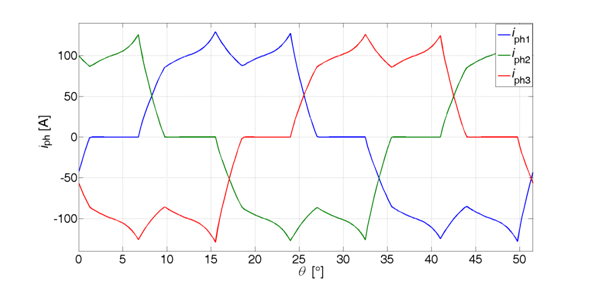
\includegraphics[width=12cm]{figures/fig2.png}
	\caption{Tytuł rysunku, rozmiar 11 pkt., pojedyncza interlinia, akapit wyśrodkowany, bez wcięcia pierwszego wiersza. Na końcu tytułu rysunku/tabeli nie stawia się kropki [8]}
\label{Fig:wykres}
\end{figure}


\begin{example}
[\ldots] oraz indukcyjności wzajemnej. W tabeli \ref{Tab:tabela} przedstawiono podstawowe parametry obwodu nieliniowego, zasilanego napięciem trójfazowym.
\end{example}

\begin{table}[ht]
\caption{Tytuł tabeli, rozmiar 11 pkt., pojedyncza interlinia, akapit wyrównany do lewej}
\centering		
	\begin{tabular}{|c|c|c|c|c|}	
		\hline
		$U$ [V] & $I$ [mA] & $R$, [k$\Omega$] & $L$ [mH] & $R/R_{20}$ \\
		\hline
		13,6 & 7,29 & 3,94 & 100 & 1,25 \\
		\hline
	\end{tabular}	
	
\label{Tab:tabela}
\end{table}	

{\subsubsection{Wzory matematyczne}}

Zmienne we wzorach pisze się czcionką pochyłą (styl edytora równań „Matematyka”) natomiast symbole, nie będące zmiennymi, czcionką prostą (styl „Tekst”).
Rozmiary czcionek: normalny 12 punktów, indeks dolny/górny 9 pkt., indeks podrzędny 7 pkt., symbol 24 pkt., podsymbol 12 pkt. Separatorem dziesiętnym w liczbach jest
przecinek, a nie kropka (dotyczy to również liczb pisanych w tekście akapitu). Poddaj się w tym zakresie \LaTeX'owi - pisz wzór, a poprawnie się utworzy.


Pod wzorem należy zamieścić objaśnienia użytych symboli (chyba, że znajdują się w wykazie na początku pracy). Wzory umieszcza się wyśrodkowane i numeruje zgodnie
z kolejnością w danym rozdziale: (numer\_rozdziału.numer\_wzoru). Numery wzorów wyrównuje się do prawego marginesu. W akapicie poprzedzającym wzór musi znajdować się krótki opis, czego dotyczy dany wzór i – jeżeli potrzeba – odwołanie do literatury.

\begin{example}
[\ldots] wyznacza się, na podstawie wyrażenia (\ref{Eq:rownanie}). W nawiasach podano rozmiary czcionek używanych we wzorach
\end{example}

\begin{equation}
A(12)={\sum}(24)m_{s(9)}N^{k_{p(7)}}
\label{Eq:rownanie}
\end{equation}
gdzie: $m_s$ -- masa próbki, $N$ -- natężenie oświetlenia, $k_p$ -- wykładnik potęgi $(k_p=1,3-2,1)$.\\
\newpage
{\subsubsection{Listingi programów}}

W pracy dyplomowej możesz umieszczać fragmenty programów. Pamiętaj, aby umieszczać krótkie, tylko najważniejsze fragmenty kodów źródłowych. Zawsze je komentuj w treści
pracy dyplomowej. Typowo w \LaTeX\ kody źródłowe umieszczane są w środowisku verbatim (\verb|\begin{verbatim}...\end{verbatim}|). Obecnie instnieje jednak bardziej nowoczesne i bardziej funkcjonalne środowisko \verb|lstlisting| (wymaga zainstalowanego w systemie pakietu \verb|listings|). Zwróć uwagę, że możesz kolorować składnię
automatycznie za pomocą parametru \verb|language|. W niniejszym dokumencie przedstawiono dwa przykłady listingów, Listing \ref{KodMatlab1} to przykład kodu źródłowego Matlaba, a poniżej Listing \ref{KodPerl1} dla Perl'a.\\
%\komentarz{

\begin{lstlisting}[language=Matlab,caption=Listing programu Matlab,label={KodMatlab1}]
i = 1
p = 3
for i = 1:10
    if i > 3
        i=i+p
    else 
        i=i+1
    end
end
\end{lstlisting}

\begin{lstlisting}[language=Perl,caption=Listing programu Perl,label={KodPerl1}]
  my $url ='http://pei.prz.edu.pl';
  use LWP::Simple;
  my $content = get $url;
  die "Couldn't get $url" unless defined $content;
  print $content;
  print "\n";
  print "Length " + length($content)
\end{lstlisting}

Z pewnością przeglądając źródło tego dokumentu zobaczysz, że kody źródłowe powinny mieć zdefiniowane parametry \verb|label|, aby łatwo w tekście do nich się odwoływać.
Numeracja linii jest w stylu domyślnie włączona (to przydatne, bo w treści pracy łatwo odwołać się dzięki temu do konkretnego wiersza w kodzie źródłowym), możesz je wyłączyć podając jako parametr \verb|numbers=none|. Więcej szczegółów możesz odnaleźć w sekcji \verb|\lstset| pliku arkusza styli. 
%}


\subsubsection{Numerowanie i punktowanie}

\begin{enumerate}[label=\arabic*), leftmargin=1.25cm]
	\item Pierwszy poziom (stosuje się numerowanie lub punktowanie). Formatowanie:
	akapit wyjustowany, wcięcie od lewej 0,75 cm, wysunięcie co 0,5 cm.
	\item Znakiem numerowania jest liczba (z kropką lub nawiasem).
		\begin{itemize}[label=-,labelsep=0.4cm,leftmargin=0.6cm]
			\item drugi poziom (stosuje się wyłącznie punktowanie). Formatowanie: akapit
			wyjustowany, wcięcie od lewej 1,25 cm, wysunięcie co 0,5 cm,
			\item znakiem punktowania jest łącznik lub mała litera alfabetu (z nawiasem). Nie
			zaleca się stosowania kropek, strzałek itp.,
			\item punktowane akapity rozpoczyna się minuskułą (małą literą), na końcu akapitu
			stawia się przecinek, ostatni punktowany akapit kończy się kropką.
		\end{itemize}
	\item Numerowane akapity rozpoczyna się majuskułą (wielką literą) i kończy kropką.
	\item Należy zwrócić uwagę, aby nie rozdzielać numerowania/punktowania pomiędzy
	kolejnymi stronami tekstu.
\end{enumerate}


\subsection{Wykaz literatury}

W wykazie literatury zamieszcza się wyłącznie pozycje, na które powołano się
w pracy. Kolejność numerów w wykazie – zgodna z kolejnością pojawiania się danej
pozycji w tekście.

Format akapitu: akapit wyjustowany, wysunięcie 0,75 cm. Prawidłowo opracowany
wykaz został zaprezentowany w niniejszym dokumencie w odpowiednim rozdziale, oznaczonym jako „Literatura”  (pozycja nr \cite{str} to zasoby internetowe,
\cite{Jakubczyk1997} – książka, \cite{Barski2011} – artykuł w czasopiśmie, \cite{dokum} – karta katalogowa).

{\subsection{Wydruk pracy}}

Przed wydrukiem należy usunąć ewentualne błędy literowe i sprawdzić prawidłową
interpunkcję. Przykładowo, łącznik zapisuje się za pomocą krótkiego minusa (np.
badawczo-rozwojowy) natomiast myślnik -- stosowany w zdaniach wtrąconych -- zapisuje
się za pomocą długiej pauzy. Dzielenie wyrazów według uznania Autora (można podzielić
długie wyrazy, powodujące duże „rozstrzelenie” tekstu w poprzedzającym wierszu. Zaleca się usunięcie pojedynczych znaków na końcu wiersza oraz podwójnych spacji w tekście.
Dla przedrostka „mikro” należy unikać stosowania litery „u” zamiast „$\mu$”. Znak „$\mu$” można
otrzymać przytrzymując lewy Alt i wpisując na klawiaturze numerycznej 0181 (podobnie
„stopień”: Alt-0176). W celu uniknięcia „rozstrzelenia” liczb i ich jednostek zaleca się
używanie „twardej” spacji pomiędzy liczbą i jednostką. Należy sprawdzić, czy tytuły
podrozdziałów/zakresów nie zostały jako pojedyncze wiersze na poprzedniej stronie oraz
czy rysunki/tabele i ich tytuły nie zostały rozdzielone pomiędzy kolejnymi stronami.

Pracę drukuje się dwustronnie. Zaleca się wydruk w kolorze. Przed wydrukiem
należy ponumerować strony (czcionka 10 pkt., dół strony, akapit wyśrodkowany). Strony
tytułowej oraz strony z podziękowaniem nie numeruje się. Spis treści rozpoczyna się od
strony numer 3 (lub 5, jeżeli zamieszczono podziękowania).

\clearpage

\section{Podsumowanie i wnioski końcowe}

1 $\div$ 3 stron merytorycznie podsumowanie najważniejszych elementów pracy oraz wnioski wynikające z osiągniętego celu pracy. Proponowane zalecenia i modyfikacje oraz rozwiązania będące wynikiem realizowanej pracy.

Ostatni akapit podsumowania musi zawierać wykaz własnej pracy dyplomanta i zaczynać się od sformułowania: „Autor za własny wkład pracy uważa: \ldots”.

\clearpage

\section*{Załączniki}
\addcontentsline{toc}{section}{Załączniki}

Według potrzeb zawarte i uporządkowane uzupełnienie pracy o dowolny materiał źródłowy (wydruk programu komputerowego, dokumentacja kons\-truk\-cyj\-no-\-tech\-no\-lo\-gicz\-na, konstrukcja modelu -- makiety -- urządzenia, instrukcja obsługi urządzenia lub stanowiska laboratoryjnego, zestawienie wyników pomiarów i obliczeń, informacyjne materiały katalogowe itp.).


\clearpage

\addcontentsline{toc}{section}{Literatura}

\begin{thebibliography}{4}
	\bibitem{kiaMultiLayer} http://materialy.prz-rzeszow.pl/pracownik/pliki/34/sztuczna-inteligencja-cw9-siec-wielowarstw.pdf (Dostęp 05.06.2022r.)
	\bibitem{kiaSingleLayer} http://materialy.prz-rzeszow.pl/pracownik/pliki/34/sztuczna-inteligencja-cw8-siec-jednowarstw.pdf (Dostęp 05.06.2022r.)
	\bibitem{nndl} Nielsen M.: Neural Networks and Deep Learning. http://neuralnetworksanddeeplearning.com/ (Dostęp. 05.06.2022r.)
	\bibitem{kiaAcc} http://materialy.prz-rzeszow.pl/pracownik/pliki/34/sztuczna-inteligencja-cw10-przysp-uczenia.pdf (Dostęp 13.06.2022r.)
	\bibitem{nnd} Hagan T.M., Demuth H.B., Beale M.H.: Neural Network Design. https://hagan.okstate.edu/NNDesign.pdf (Dostęp 13.06.2022r.)
\end{thebibliography}

\clearpage

\makesummary

\end{document} 
